\section{Payments}
\label{section:payments}

\begin{figure}[H]
    \centering
    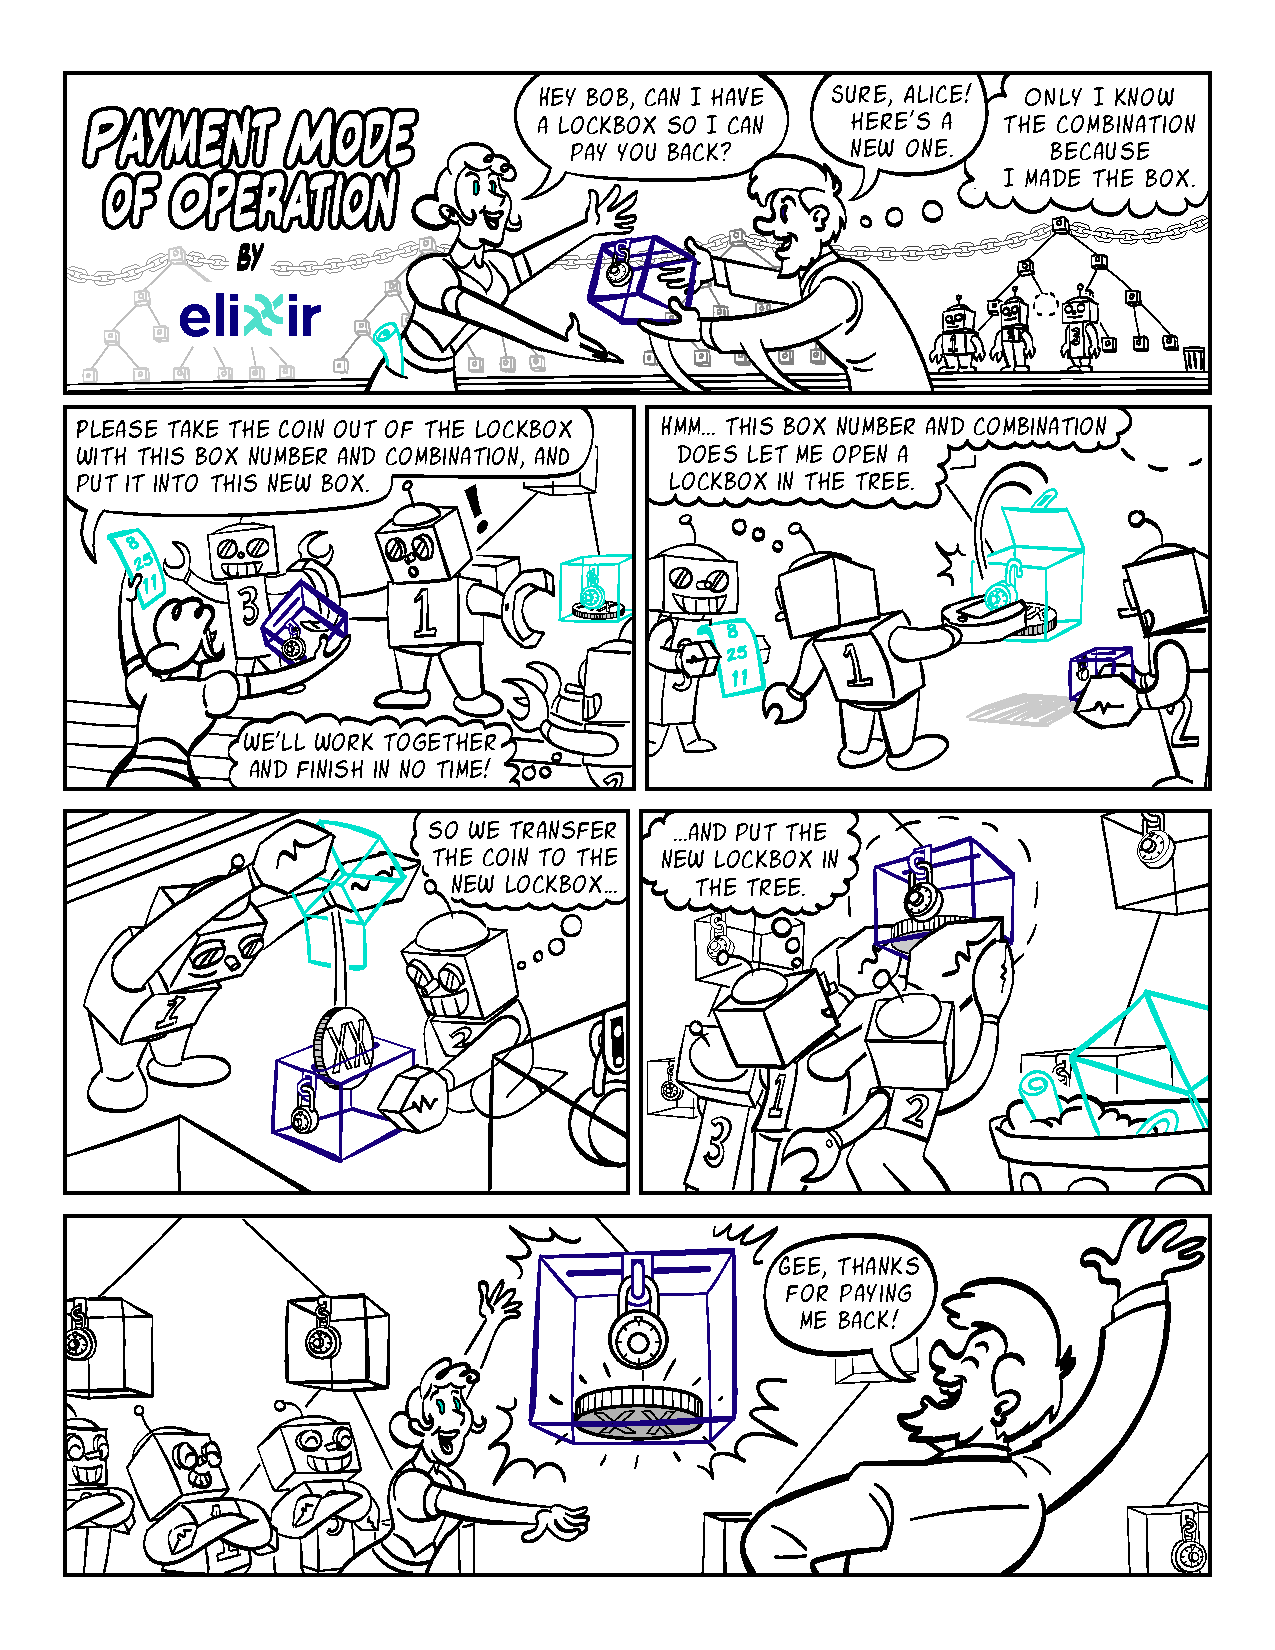
\includegraphics[width=\textwidth]{cartoons/PaymentOperation.pdf}
    %\caption{Illustration of an example transaction from Alice to Bob}
    %\label{fig:payment_cartoon}
\end{figure}

\break

Token handling in the \name platform has some unique attributes. Token handling in most conventional blockchain systems today is wallet-based. In the \name protocol, token handling is token based, meaning the token remains static, while a secret is required to prove ownership. These secrets are kept off-chain and change when ownership of a token is assigned to a new owner. 

\name secures individual tokens rather than securing an entire wallet as a whole. Each token owned by a user is secured through knowledge of an individual secret, which means that even if an attacker successfully performs a brute-force attack, only one single token from the user can be compromised.

\name blocks do not contain any information about transactions, i.e. sender, receiver, and amount. Instead, a block from the \name blockchain contains assignments of tokens to addresses belonging to the payee, and previous addresses belonging to the payer. Moreover, there is no information linking payer and payee in the blockchain, which translates into on-chain unlinkability. 

\subsection{Block Structure}

\name takes a new approach to the information contained in blocks. Each block contains nothing more than unordered lists of the past and new addresses to which tokens were assigned by the transactions of that block.

By analyzing the entire blockchain, an observer is unable to link the transacting parties or the features of the transaction to one another (i.e., how many were sent).  As a result, one can only infer that in a specific block a set of tokens have been unlinkably assigned to new addresses from old addresses.

To contextualize such block information, we show a snippet of what is present in the \name block explorer tool in Figure~\ref{fig:block_explorer}.

\begin{figure}[H]
    \centering
    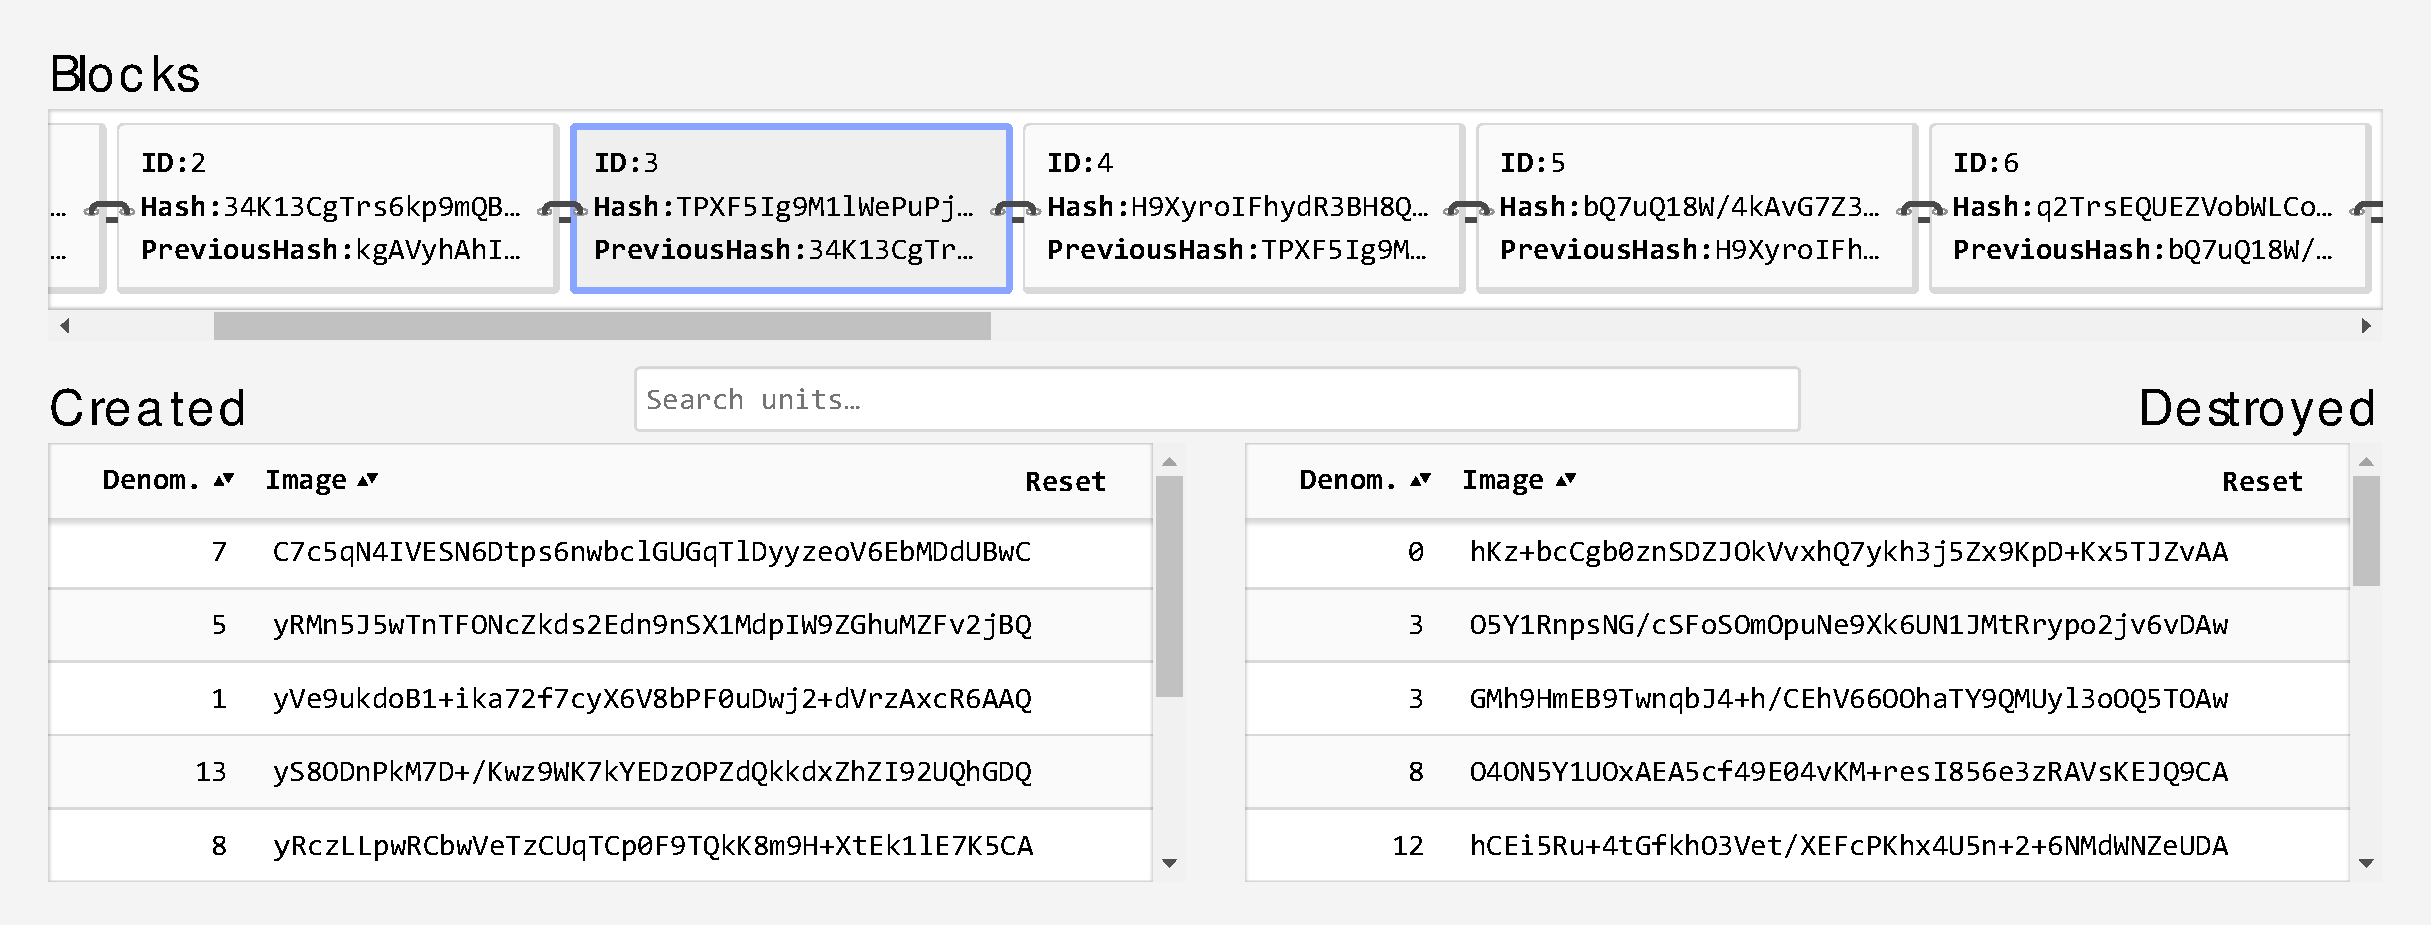
\includegraphics[width=\textwidth]{img/Block-Explorer.pdf}
    \caption{Block \#3 from the \name Block Explorer}
    \label{fig:block_explorer}
\end{figure}

Within both the block and the nodes, data is stored as a binary radix tree combined with a Merkle tree~\cite{merkle}. This structure allows for fast searching and rehashing of the root within the nodes, and for proofs to be generated that verify the existence of a token within a block. This is achieved simply by revealing the hashes of the block root, the token, and all non-leaf data blocks in between. As a result, shorthand proofs can be generated and used for validation in lieu of requiring all of the data of a relevant block referencing the transaction of interest. 

\subsection{Payment Preliminaries}

Normally, in the blockchain space, users submit a transaction---signed with their corresponding private key---to the system. The nodes in the system then check the validity of the transaction by employing the user's corresponding public key. If the key is valid and the user has funds to perform the payment, then the transaction is written to a block. 

\name introduces a new and faster concept: \textit{Hash-Based Ownership}. Since hash functions are considered infeasible to invert, users can use pre-images as proof of their ownership of specific images. By chaining this process of revealing these pre-images with our \name protocol, users are able to perform payment transactions anonymously and securely. Furthermore, this process ensures that no one is able to forge a fake transaction in an attempt to steal someone's tokens.

\subsection{Making a payment}

A simplified payment transaction in the system starts with an invoice. Bob sends Alice an invoice containing the destination address (where she should send the money). This address is an image (the output of a hash function) that Bob previously generated from a random preimage (a secret that is the input to a hash function).
    
Alice, after receiving the destination image (address), submits a payment transaction to the system. This transaction contains the preimage (secret) of a token she owns along with the image (address) from Bob's invoice.
    
The system checks whether the preimage (secret) Alice sent is valid and exists in the ledger and then transfers the specified amount from Alice's token to Bob's destination image (address). After processing the transaction successfully, the system returns a proof receipt to Alice that she can share with Bob, which validates that the transaction executed correctly.

This receipt provides proof that the transaction is properly recorded in the block by providing the Merkle path within the block of those tokens. This alone is enough proof that the transfer took place correctly and that, therefore, the tokens now belong to Bob. However, both parties (Alice or Bob) can freely check the blockchain and verify that the destination image (address) and the proper amount are present in the corresponding block.

\name's unique architecture and payment processing mechanisms offer three advantages over traditional approaches:

\begin{enumerate}
    \item User confidentiality is protected by the limited information that is available on-chain. 
    \item Security is increased substantially by securing tokens instead of wallets. In the exceptionally rare event that a successful brute-force attack does occur, security of at most one token may be affected. 
    \item Transaction processing is faster because hash-based ownership can be completed in a fraction of the time required for a digital signature in traditional blockchain platforms. 
 \end{enumerate}  
    
As others have said~\cite{sphincs}, when contrasting digital signatures characteristic of traditional blockchain platforms to hash-based digital signatures used in the \name platform, ``\textit{Every signature scheme uses a cryptographic hash function; hash-based signatures use nothing else}''  Lastly, unlike digital signatures, hashes are secure against quantum-computational capabilities.


